\documentclass{article}
\usepackage{tikz}
\usetikzlibrary{arrows.meta, quotes}

\begin{document}

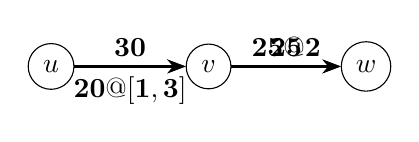
\begin{tikzpicture}[node distance = 2cm, auto]
    \node [circle, draw] (u) {$u$};
    \node [circle, draw, right of=u] (v) {$v$};
    \node [circle, draw, right of=v] (w) {$w$};

    \path[->, thick, >=Stealth]
        (u) edge ["$\mathbf{20@[1,3]}$" '] (v)
        (v) edge ["$\mathbf{25@2}$"] (w)
        (u) edge ["$\mathbf{30}$", below left] (v)
        (v) edge ["$\mathbf{25}$", below right] (w);
\end{tikzpicture}

A simple instance of the Interval Debt Model (IDM). Numbers in square boxes represent the assets of the nodes (for example, €30 for node \( u \)), directed edges represent debts, and the labels on the edges indicate the terms of the associated debts (for example, node \( u \) must pay node \( v \) €20 between times 1 and 3).

\end{document}